\documentclass[12pt]{article}

\usepackage[spanish]{babel}
\selectlanguage{spanish}
\usepackage[utf8]{inputenc}
\usepackage{vmargin}
\usepackage{graphicx}
\setmargins{2.5cm}{1.5cm}{16.5cm}{23.42cm}{0pt}{1cm}{0pt}{2cm}

\title{Tiro Parabólico}
\author{Martín Alejandro Paredes Sosa}
\date{Abril 2015}
\graphicspath{{IMG/}}

\begin{document}
\maketitle

\section{Introducción}
En la realización de esta práctica, se estudió el tiro parabólico cuando existe una resistencia, la que en este caso es el aire. Utilizando las ecuaciones de movimiento para tiro parabólico con resistencia en el aire, se realizó un programa en FORTRAN, donde el usuario ingresa la posición del proyectil esférico, velocidad inicial y ángulo de tiro, con los cuales nos permite calcular la posición en diferentes tiempos, su alcance, altura máxima y el tiempo total de vuelo en un tiro con y sin resistencia al aire.

\section{Código}
En este apartado se mostrara el código FORTRAN y la manera en que funciona.
\subsection{Algoritmo}
El programa consiste:
	\begin{enumerate}
	\item Ingreso de datos por usuario:  Posición $x$ y $y$, Ángulo y velocidad del proyectil
	\item Se ingresa a la subrutina de nFric
	\item El ángulo es convertido a radianes, con el cual se descompone la velocidad en $x$ y $y$.
	\item Se crea un documento $nfric.dat$ donde se escribirá la posición del proyectil.
	\item Se inicia un ciclo donde se calcula la posición en ambos ejes coordenados
	\item Cuando la altura llega a 0 se termina el ciclo y se calcula el alcance y altura máxima.
	\item Se ingresa a la subrutina de Fric
	\item El ángulo es convertido a radianes
	\item Se pide la masa del proyectil y el radio
	\item Se crea el documento $Fric.dat$ donde se escribirá la posición del proyectil.
	\item Se inicia un ciclo donde se calcula la posición $x$ y $y$.
	\item Cuando la altura llega a 0 se termina el ciclo y se calcula el alcance y altura máxima.
	\item Se imprimen resultados en pantalla de alcance, altura máxima y tiempo total de vuelo.
\end{enumerate}

\subsection{Código FORTRAN}
\begin{verbatim}
!===================================================================
!Este programa calcula el tiro parabolico con resistencia en el aire
!===================================================================
!===================================================================
MODULE cons

  Real , parameter :: grad =(4*atan(1.0))/180
  Real , parameter :: pi=4*atan(1.0)
  Integer , parameter :: ntps = 6000
  Real , parameter :: g = 9.806

  Real , parameter :: DAire = 1.29 !Densidad del aire
  Real , parameter :: Csphere = 0.47
END MODULE cons
!===================================================================
subroutine nFric (xi,yi,vi,ang,xnf,ynf,tnf)
 
  USE cons
  IMPLICIT NONE
  Integer :: i 
  Real, Dimension (1:ntps) :: x,y,t
  Real :: xi, yi, vi, ang,rad    !Variables externas
  Real :: xnf, ynf, tnf    !Variables internas

  rad = ang*grad !conversion Grad-Rad

  tnf = (2*vi*SIN(rad))/(g)
  xnf = xi+((vi*vi+SIN(2*rad))/(g))
  ynf = yi+(((vi*vi)*(SIN(rad)*SIN(rad)))/(2*g))

  OPEN (1, FILE = "nfric.dat")

  DO i=1,ntps,1

    IF (ang==0) THEN
	tnf = 0
	xnf = 0
	ynf = 0
	y(i)= 0
	t(i)= float(i)*0.01	
	x(i)= 0
    ELSE IF (ang==90) THEN
	tnf = (2*vi*SIN(rad))/(g)
	xnf = 0
	ynf = yi+(((vi*vi)*(SIN(rad)*SIN(rad)))/(2*g))		
	t(i)= float(i)*0.01
	x(i)=0
	y(i)= yi + (vi * sin(rad) *t(i)) - (0.5*g*t(i)*t(i))
    ELSE 
	tnf = (2*vi*SIN(rad))/(g)
	xnf = xi+((vi*vi+SIN(2*rad))/(g))
	ynf = yi+(((vi*vi)*(SIN(rad)*SIN(rad)))/(2*g))	
	t(i)= float(i)*0.01
	x(i)= xi + (vi * cos(rad) *t(i))
	y(i)= yi + (vi * sin(rad) *t(i)) - (0.5*g*t(i)*t(i))
    END IF     
     
     write (1,1001) x(i), y(i)
     1001 format (f11.5,f11.5)
 

  IF (y(i)<0) EXIT
     
  END DO

  CLOSE (1)
  
end subroutine nFric
!===================================================================
subroutine Fric (xi,yi,vi,ang,xf, yf, tf)
	
	USE cons
	IMPLICIT NONE
	integer :: i
	REAL, DIMENSION (0:ntps) :: ax, dy, ct, velax, velby, aax, aby
	Real :: xi, yi , vi, ang, rad !Entrada
	Real :: xf, yf, tf  !Salida
	Real :: area , radio, masa , ad
	
	Print *, 'Ingrese la masa del objeto (kg)'
	Read *, masa
	Print *, 'Ingrese el radio del proyectil'
	Read *, radio
	area= pi*radio*radio
	rad = ang*grad
	!do i=0 , ntps ,1	 Ignorar
		!by(i)=0         Debug Problema  con los valores dentro del array
	!end do			 No hacer caso a esto
	
	ax(0) = xi
	dy(0) = yi
	velax(0) = vi*cos(rad)
	velby(0) = vi*sin(rad)
	ad = (0.5*DAire*Csphere*area)/masa
	aax(0) = -ad*velax(0)*velax(0)
	aby(0) = -g-(ad*velby(0)*velby(0))
	ct(0) = 0

	OPEN(2, FILE="Fric.dat")
	write (2,1001) ax(0), dy(0)
	1001 format (f11.5,f11.5)

	DO i=0, ntps, 1
          IF (ang==0) THEN
	    ct(i+1) = 0 
	    ax(i+1) = 0 
	    dy(i+1) = 0 
          ELSE IF (ang==90) THEN
	    ct(i+1) = ct(i)+0.01
	    velby(i+1) = velby(i)+ aby(i)*ct(i+1)
	    aby(i+1) = -g-(ad*velby(i)*velby(i))
	    ax(i+1) = 0 
	    dy(i+1) = dy(i)+ velby(i)*ct(i+1)+ (0.5*aby(i)*ct(i+1)*ct(i+1))
          ELSE 
	    ct(i+1) = ct(i)+0.01
	    velax(i+1) = velax(i)+ aax(i)*ct(i+1)
	    velby(i+1) = velby(i)+ aby(i)*ct(i+1)
	    aax(i+1) = -ad*velax(i)*velax(i)
	    aby(i+1) = -g-(ad*velby(i)*velby(i))
	    ax(i+1) = ax(i)+ velax(i)*ct(i+1)+ (0.5*aax(i)*ct(i+1)*ct(i+1))
	    dy(i+1) = dy(i)+ velby(i)*ct(i+1)+ (0.5*aby(i)*ct(i+1)*ct(i+1))
          END IF     
	    	
	  write (2,1001) ax(i+1), dy(i+1)
	  IF (dy(i+1)<0) EXIT
	END DO
	
	CLOSE(2)
	xf = ax(i+1)
	yf = MAXVAL(dy)
	tf = ct(i+1) * 10.0
        
	!do i=0 , ntps ,1		Ignorar
		!print *, dy(i+1)	Debug Problemas con el array
	!end do				No hecer caso a esto 
	
end subroutine Fric
!===================================================================
program proyectil
  use cons
  implicit none
  !Declaración
  Real:: xi, yi, vi, ang !Entrada
  Real:: xnf, ynf, tnf, xf, yf, tf      !Salida
  Real:: error, ag
  
  PRINT *, "Este programa calcula el tiro parabolico con resistencia "
  PRINT *, "y sin resistencia de un objeto esferico"  

  write (*,*) 'Ingrese posicion en "x","y","Vo" y Angulo'
  read *, xi, yi ,vi, ang
  ag=ang     
  call nFric (xi, yi, vi, ang, xnf, ynf, tnf)
  call Fric (xi, yi, vi, ang, xf, yf, tf)
 
  error= ((xnf-xf)/xnf) * 100.0

  PRINT *, "=========================================================="
  PRINT *, "Posicion inicial del tiro: x=", xi,", y=",yi
  PRINT *, "Con una velocidad inicial de", vi, "m/s"
  PRINT *, "Angulo de", ang, "radianes o ", ag ,"grados respecto al piso"
  PRINT *, "=========================================================="
  PRINT *, "              Sin Friccion"
  PRINT *, "El tiempo total de vuelo es:", tnf, "s"
  PRINT *, "La altura maxima alcanzada es:", ynf, "m"
  PRINT *, "Tiene un alcance de:", xnf, "m"
  PRINT *, "=========================================================="
  PRINT *, "              Con Friccion"
  PRINT *, "El tiempo total de vuelo es:", tf, "s"
  PRINT *, "La altura maxima alcanzada es:", yf, "m"
  PRINT *, "Tiene un alcance de:", xf, "m"
  PRINT *, "=========================================================="
  PRINT *, "La diferencia porcentual entre ambos tiros es", error, "%"
end program proyectil

\end{verbatim}
\pagebreak
\section{Resultados}
En este apartado se mostrara los resultados obtenidos por el .
\subsection{Tiro 0 Grados}
\begin{center}
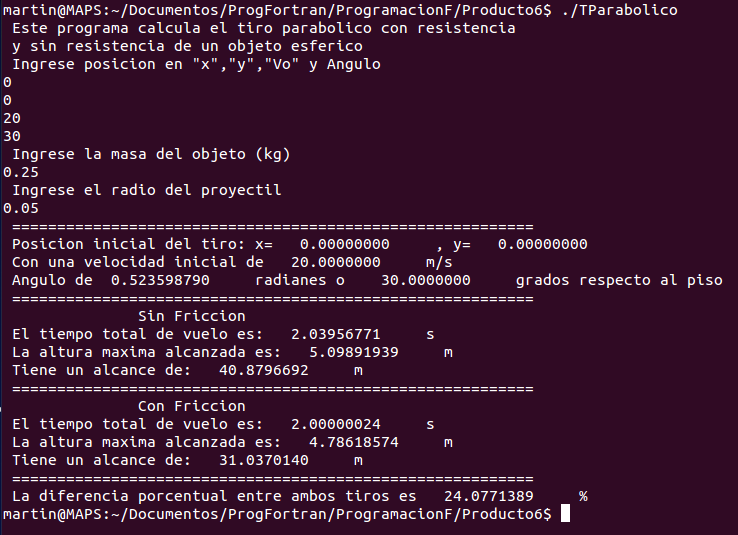
\includegraphics[width=15cm]{Tiro30g20v.png}
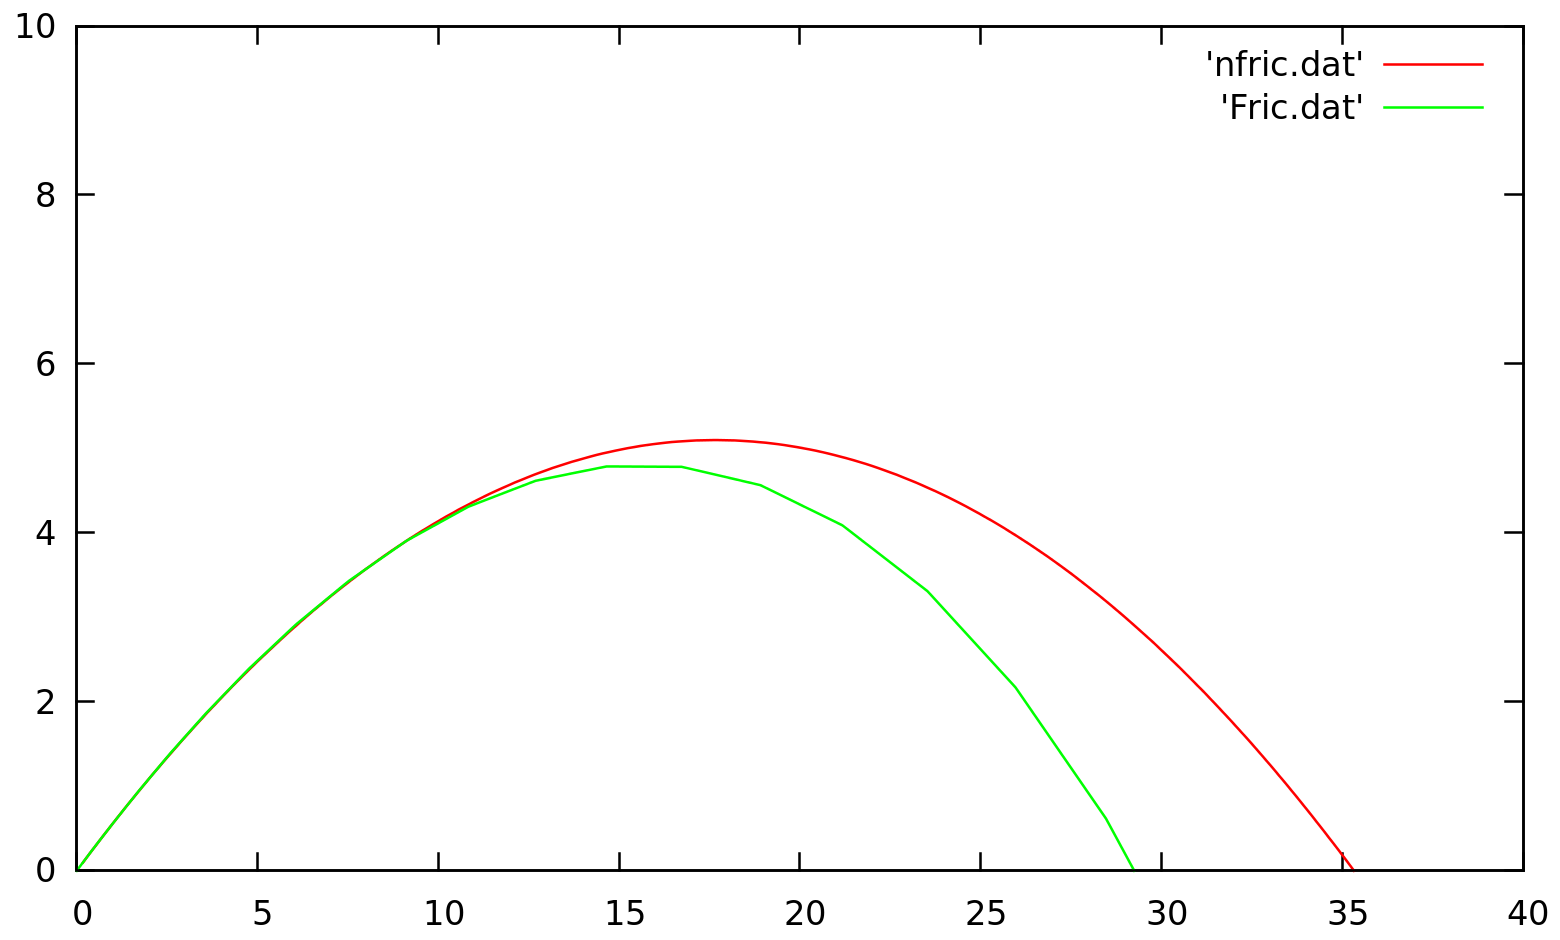
\includegraphics[width=15cm]{Tiro30g.png}
\end{center}
\subsection{Tiro 30 Grados}
\begin{center}
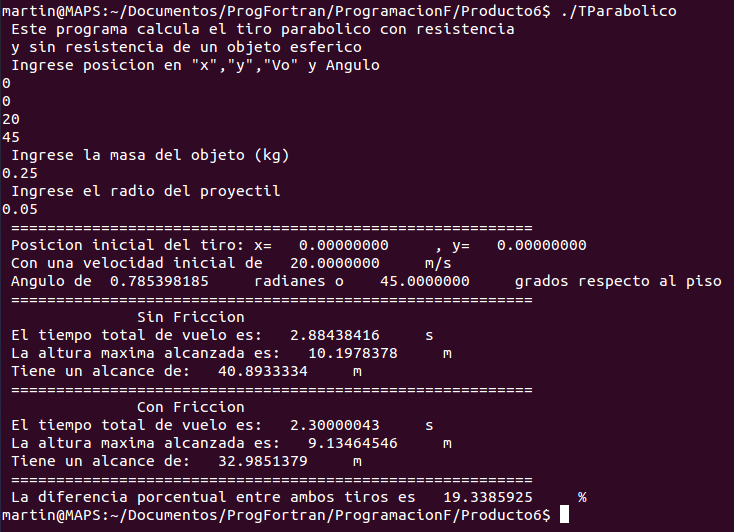
\includegraphics[width=15cm]{Tiro45g20v.png}
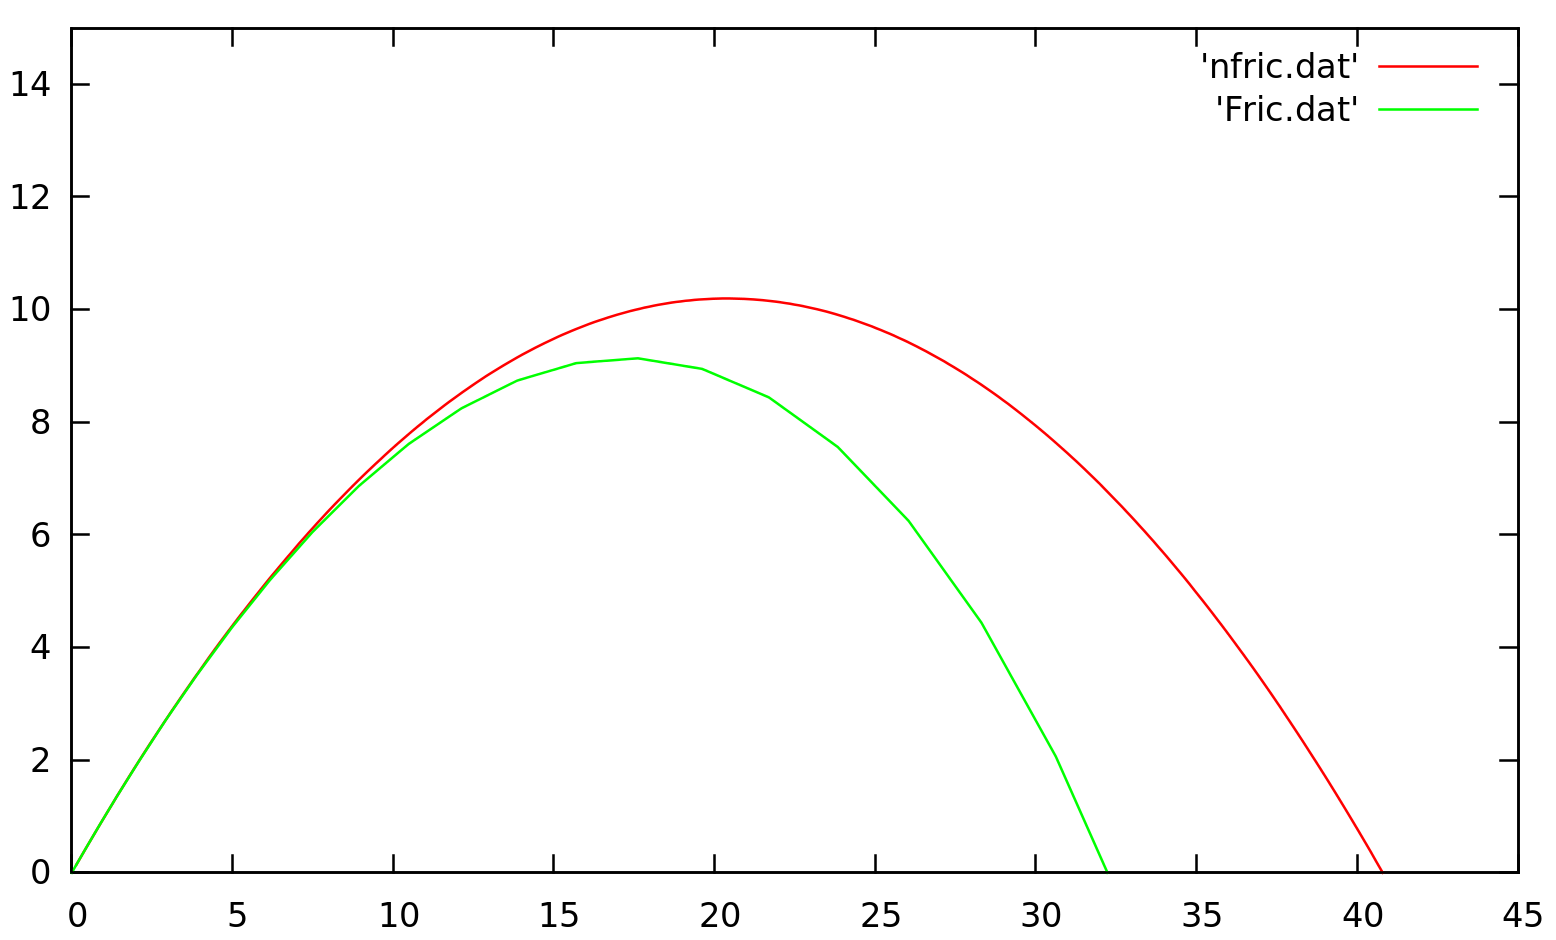
\includegraphics[width=15cm]{Tiro45g.png}
\end{center}
\subsection{Tiro 60 Grados}
\begin{center}
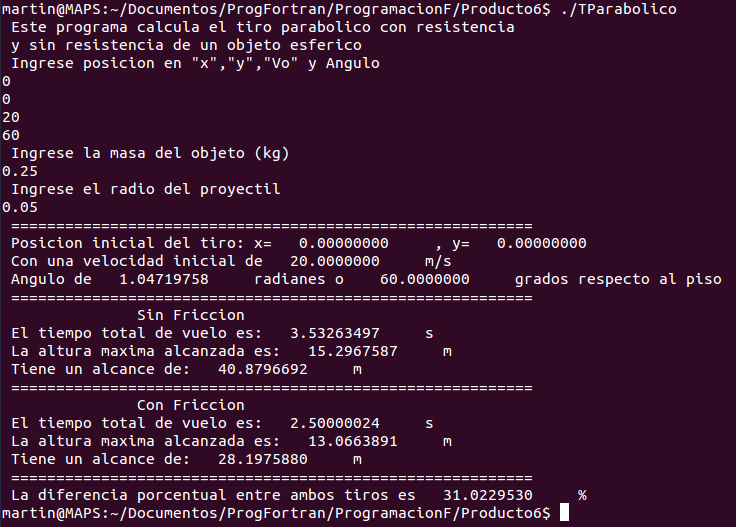
\includegraphics[width=15cm]{Tiro60g20v.png}
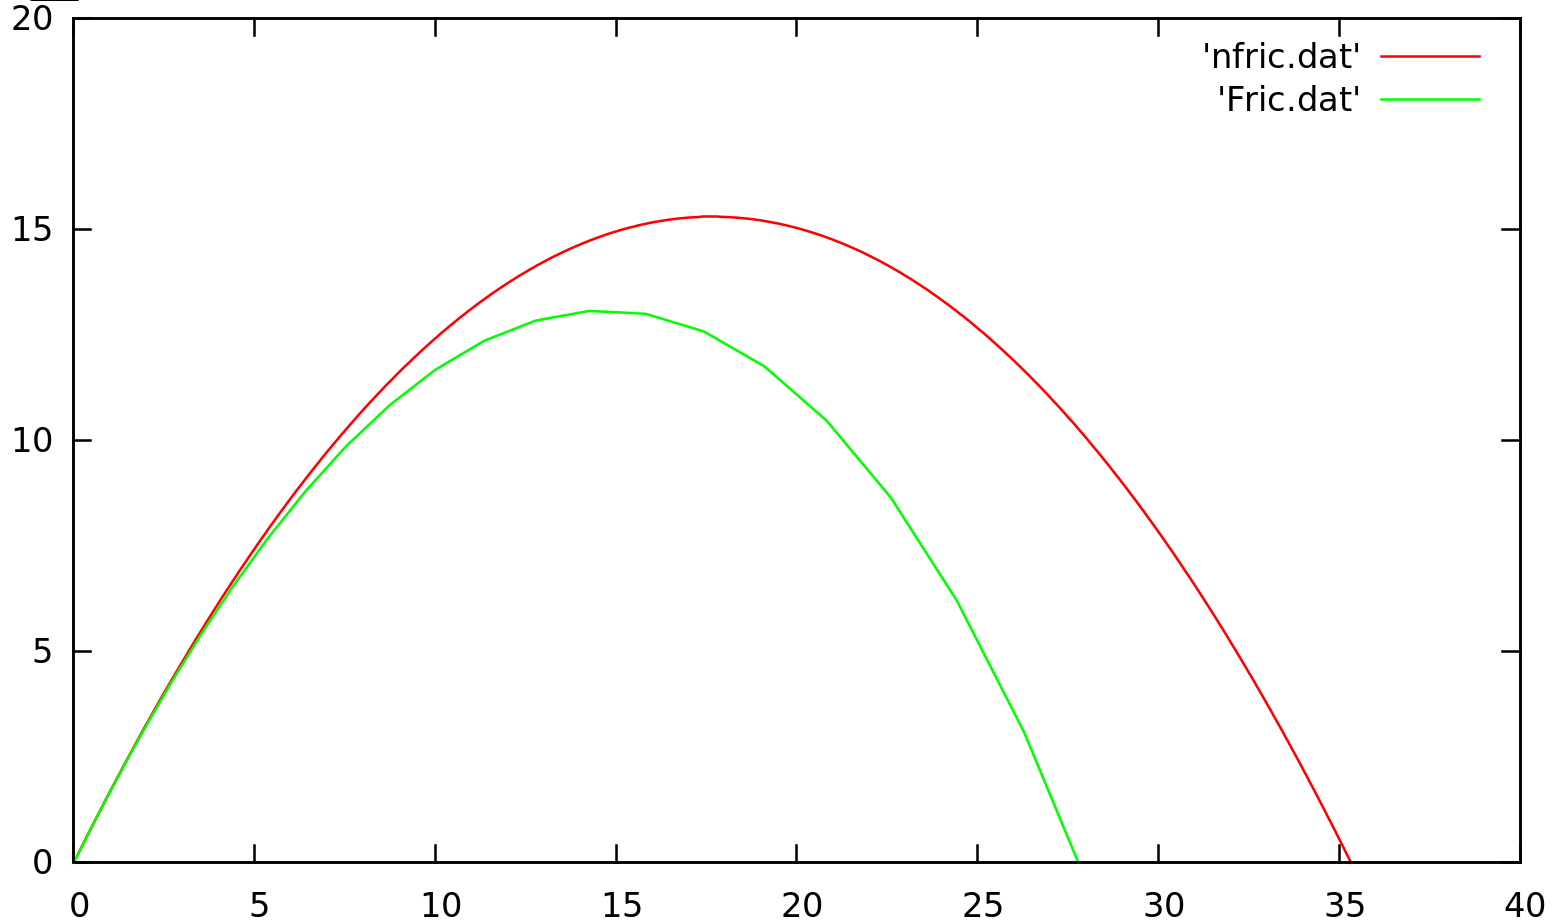
\includegraphics[width=15cm]{Tiro60g.png}
\end{center}

\end{document}
